\documentclass[a4paper, 12pt]{article}
\usepackage{matnoble-doc-en}


\begin{document}

\title{\bf {CHEM400/740: Quantum Mechanics in Chemistry\\ Chapter\#03}} \author{\bf
  \href{http://scienide2.uwaterloo.ca/~nooijen/website_new_20_10_2011/About.html}{Marcel Nooijen}} \date{}
  
\pagestyle{fancy} \fancyhead[L]{\textcolor{PrimaryColor}{CHEM400/740: Quantum Mechanics in Chemistry}} \fancyhead[R]{\textcolor{PrimaryColor}{2021 Winter}}


\maketitle
\tableofcontents

\clearpage


\section{Symmetric and Anti-symmetric Representations}
\subsection{Transpositions}
The use of transpositions allows us to characterize the fully symmetric and fully anti-symmetric representation.\\
\tab Transposition: $T_{ij}$.\\
\tab Interchange coordinates of two particles $i$ and $j$:
\begin{IEEEeqnarray}{rLl}
\hat{T}_{ij}\psi(1,2,\ldots, i, \ldots,j,\ldots,N ) =\psi(1,2,\ldots, j, \ldots,i,\ldots,N )
\end{IEEEeqnarray}
\tab Any permutation is a product of transpositions. The number of transpositions is either even or odd.\\  
\tab Parity of permutation with $P_i = 0,1$: $\hat{P}_i \longrightarrow (-)^{P_i} $\\
\tab Two types of functions represent the permutation group.
\begin{itemize}
	\item [1)] Symmetric transposition:
\begin{IEEEeqnarray}{rLl}
\hat{T}_a |\psi^{(S)}\rangle &= |\psi^{(S)}T_a(1,2,\ldots ,N)\rangle \notag \\
&= +  |\psi^{(S)}\rangle
\end{IEEEeqnarray}
The symmetric functions are he same under interchange of two coordinates.
	\item [2)] Anti-symmetric transposition: 
\begin{IEEEeqnarray}{rLl}
\hat{T}_a |\psi^{(A)}\rangle &= |\psi^{(A)}T_a(1,2,\ldots ,N)\rangle \notag \\
&= -  |\psi^{(A)}\rangle
\end{IEEEeqnarray}	
Antisymmetric functions change sign under interchange of two coordinates. \\
eg, $\psi(3,2,1)=-\psi(1,2,3)$\\
Since any permutation is a product of transpositions.
\begin{IEEEeqnarray}{rLl}
\hat{P}_k|\psi^{(S)}\rangle &= +|\psi^{(S)}\rangle \\
\hat{P}_k|\psi^{(A)}\rangle &= (-)^{\text{\# of Transp}}|\psi^{(A)}\rangle \notag \\
&= (-)^{P_k}|\psi^{(A)}\rangle
\end{IEEEeqnarray}

\end{itemize}

One can argue that one can expect this behaviour, by examining eigenfunctions of $\hat{T}$.\\
\tab Eigenfunctions of $\hat{T}$: 
\begin{IEEEeqnarray}{rLl}
\hat{T}&=\hat{T}^{-1}=\hat{T}^\dagger \\
\hat{T}| \psi\rangle &= \lambda| \psi \rangle \\
\hat{T}\hat{T}| \psi\rangle &= \lambda^2| \psi \rangle =| \psi \rangle \qquad (\hat{T}^2=1)\\
\Longrightarrow \lambda &=1 \quad \text{or} \quad \lambda=-1 \notag
\end{IEEEeqnarray}
NOTE: \\
\tab $\hat{T}$ is Hermitian and its own inverse.

 Since $\hat{T}_a$ commutes with $\hat{H}$, $\hat{T}_a|\psi\rangle$ can be chosen either to change sign or stay the same. In practice, I can make a set of commuting, $\hat{T}_{12}, \hat{T}_{34}, \hat{T}_{56}$, and demand that $\psi$ is eigenstate of $\hat{H}$ and selected $\hat{T}$. Then, one could choose some $\hat{T}_a$ to have some $\lambda_a=+1$ and some $\hat{T}_a$ to have $\lambda_a=-1$. Such eigenfunctions do exist. However, for $|\psi^{(S)}$, we can get $\hat{T}_a| \psi^{(S)} \rangle =+|\psi^{(S)}\rangle$ for all $\hat{T}_a$. For $|\psi^{(A)}$, we can get $\hat{T}_a|\psi^{(A)}\rangle =-|\psi^{(A)}\rangle$. These are the only 1-dimensional irreps of the permutation group.

Lowest degree of representation (degeneracy of $\hat{H}$):\\
\tab 1 for Symmetry(S) or Anti-symmetry(A)\\
\tab (N-1) for N-particles\\
\tab eg, if 20 electrons $\Longrightarrow$ 19-fold degeneracy (Not obscured in nature)

\subsection{Projector}
To describe fully symmetric or anti-symmetric wave functions projectors are useful. 
\begin{figure}[H]
        \centering
        % 1
        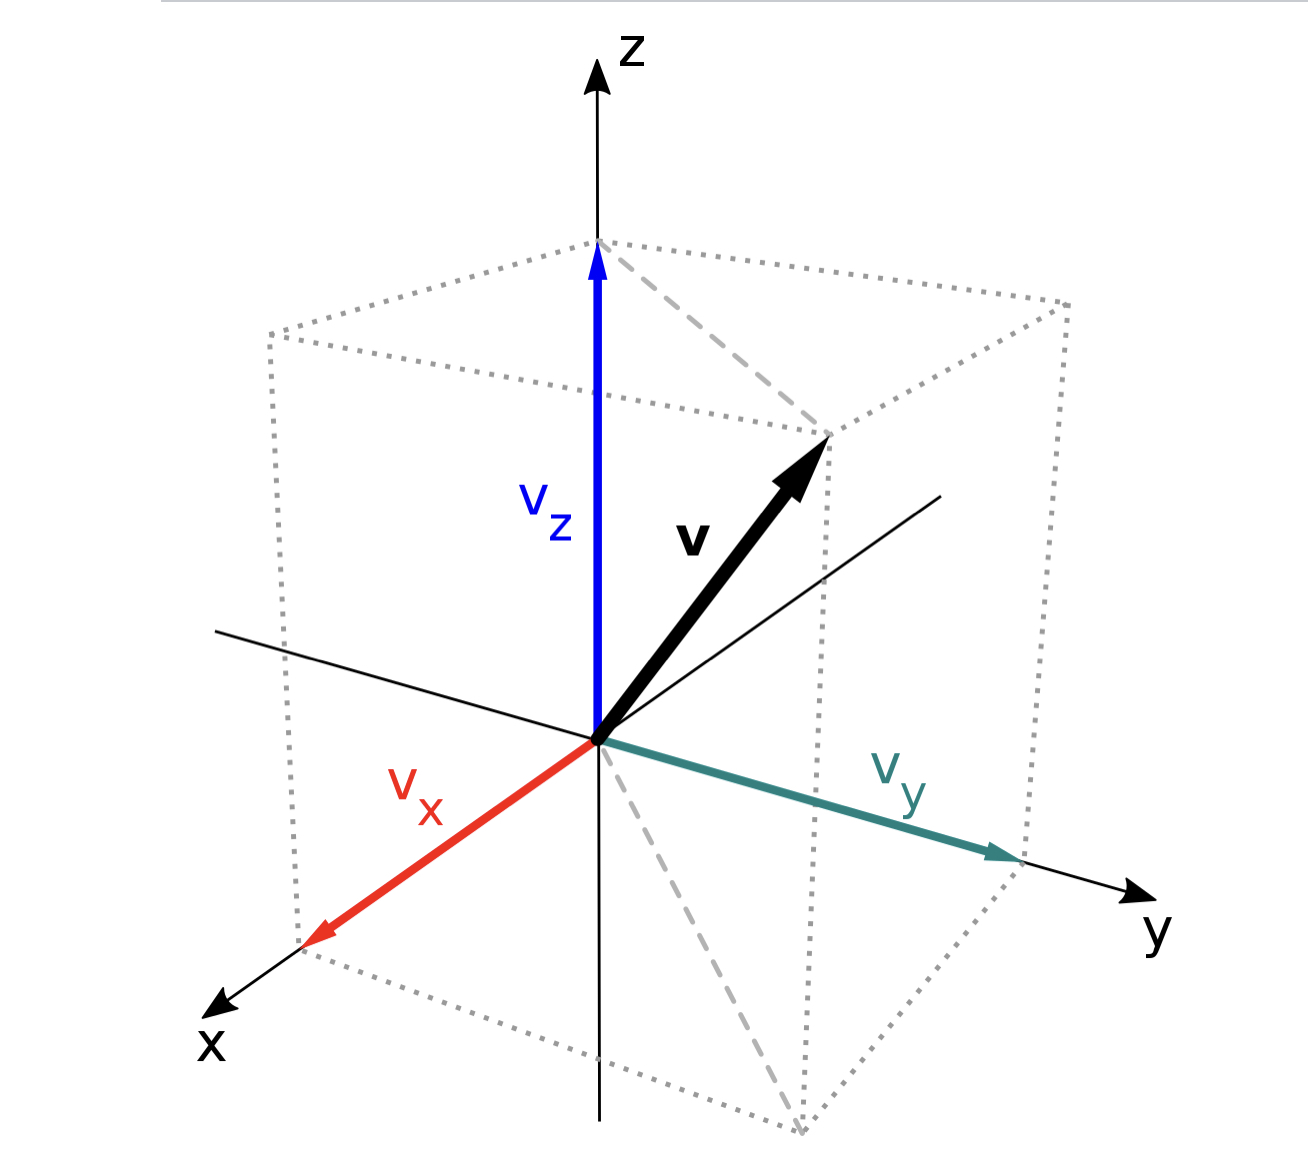
\includegraphics[width=.3\linewidth]{01.jpg}
        \caption{Projector on the x,y,z axis}
        \label{fig:sub-first2}
\end{figure}
$\hat{P}_{xy}$: projector on the xy-plane.\\
\tab Eigenvectors: \\
\tab Vector onto z-axis:  $\hat{P}\hat{e}_z\cdot a =0 \Longrightarrow \lambda=0$.\\
\tab Vector in the xy-plane: $\hat{P}_{xy}(a\vec{e}_x+b \vec{e}_y) =a\vec{e}_x+b \vec{e}_y \Longrightarrow \lambda=1 $

For an orthogonal projector:
\begin{IEEEeqnarray}{rLl}
p^2=p \\
p^\dagger = p
\end{IEEEeqnarray}
\tab Eigenfunctions of a projector:
\begin{IEEEeqnarray}{rLl}
p|\psi\rangle &=\lambda|\psi\rangle \\
p^2|\psi\rangle &= p \cdot p|\psi\rangle =\lambda^2| \psi \rangle \notag \\
&= p|\psi\rangle =\lambda | \psi\rangle \\
\Rightarrow &(\lambda^2-\lambda )|\psi\rangle = 0 \\
\Rightarrow & \lambda =1 \quad \text{or} \quad \lambda=0 \notag
\end{IEEEeqnarray}
\tab $\hat{p}|\psi\rangle =|\psi\rangle$: \\
\tab \tab \tab \tab  $|\psi\rangle$ is in the subspace defined by $\hat{p}$.\\
\tab \tab \tab \tab  $\hat{p}(\hat{p}|\psi\rangle )$ is  eigenvector of $\hat{p}$ with eigenvalue of 1.\\
\tab $\hat{p}|\psi\rangle=0$: \\
\tab \tab \tab \tab  $|\psi\rangle$ is orthogonal to subspace defined by $\hat{p}$.\\
\tab \tab \tab \tab $\hat{p}=\sum_{\lambda \in \text{subspace}}|\phi_\lambda\rangle \langle \phi_\lambda |$ with $\langle \phi_\lambda|\phi_\mu\rangle =\delta_{\lambda\mu}$.\\
\tab \tab \tab \tab  |ket$\rangle\langle$bra| is related to projector. $|\phi_\lambda\rangle$ is  orthonormal basis for subspace.\\

\subsection{Symmetric and Anti-symmetric Representations}
Here we define projectors on the symmetry(S) and anti-symmetry(A) subspace.
\begin{IEEEeqnarray}{rLl}
\hat{S} &= \frac{1}{N!}\sum_{k=1}^{N!}\hat{P}_k \\
\hat{A} &= \frac{1}{N!}\sum_{k=1}^{N!}(-)^{P_k}\hat{P}_k 
\end{IEEEeqnarray}
\tab In the exercise you will proof that $\hat{S}/\hat{A}$ are Hermitian and that they satisfy $\hat{S}^2=\hat{S}; \hat{A}^2=\hat{A}$. $\hat{p}^2=\hat{p}$ is called idempotent.\\
\tab Let us proof that $\hat{A}|\psi\rangle$ is fully antisymmetric, irrespective of $|\psi\rangle$.
$\Rightarrow$ To proof: $\hat{T}_a(\hat{A}|\psi\rangle )=-\hat{A}|\psi\rangle$
\begin{IEEEeqnarray}{rLl}
\hat{T}_a (\hat{A}|\psi\rangle )&=\hat{T}_a\frac{1}{N!}\sum_{k=1}^{N!}(-)^{P_k}\hat{P}_k|\psi\rangle \notag \\
&= \frac{1}{N!}\sum_{k=1}^{N!}(-)(-)^{P_k+1}(\hat{T}_a\hat{P}_k)|\psi\rangle
\end{IEEEeqnarray}
\tab NOTE:\\
\tab \tab $(-)(-)^{P_k+1}=(-)^{P_k}$.

 Now $\hat{T}_a\hat{P}_k=\hat{P}_l$ with parity $(-)^{P_k+1}=(-)^{P_l}$. Moreover, $\hat{T}_a\hat{P}_k$ runs over all permutations again. Hence: 
\begin{IEEEeqnarray}{rLl}
\hat{T}_a (\hat{A}|\psi\rangle )&=(-)\frac{1}{N!}\sum_{l=1}^{N!}(-)^{P_l}\hat{P}_l|\psi\rangle \notag \\
&= -A|\psi\rangle \qquad \forall \hat{T}_a
\end{IEEEeqnarray}
\tab NOTE:\\
\tab \tab $\sum_k\hat{P}_i\hat{P}_k=\sum_l\hat{P}_l \quad \forall k$. \\
\tab\tab This argument is always true for a fixed $\hat{P}_i$. Also, this is a crucial argument in all these proofs.

If one applies the antisymmetrized $\hat{A}$ to a product of orbitals, one gets:
\begin{IEEEeqnarray}{rLl}
\hat{A}(\phi_a(1)\phi_b(2)\cdots \phi_z(N) )&= \frac{1}{N!}\sum_{k=1}^{N!}(-)^{P_k}\hat{P}_k(\phi_a(1)\phi_b(2)\cdots \phi_z(N) ) \notag \\
&= \frac{1}{N!}|\phi_a\phi_b\cdots \phi_z  |
\end{IEEEeqnarray}
\tab The antisymmetrizer provides a generalization to the Slater determinant concept as it can be applied to any function, $\psi(1,2,\cdots,N)$. Not only to a product of orbitals.\\
\tab In chapter 2 S\&O, we use $\hat{A}$ with a different normalization.
\begin{IEEEeqnarray}{rLl}
\hat{A}'=\sum_{k=1}^{N!}(-)^{P_k}\hat{P}_k
\end{IEEEeqnarray}
\tab Then, since $\frac{1}{N!}\hat{A}'\cdot\frac{1}{N!}\hat{A}'=\frac{1}{N!}\hat{A}' $, it follows $\hat{A}'\hat{A}'=N!\hat{A}'$. $\hat{A}'$ is no longer a projector (but simpler to use).

\begin{summary}{}{}
\begin{center}
	$\left[ \hat{H},\hat{P}_k \right]=0 \qquad \hat{P}_k^\dagger \hat{P}_k=1$
\end{center} 
\tab $\hat{P}_k$ forms a symmetric group, $S_N, k=1\cdots N!$.\\
\tab This implies that eigenfunctions of $\hat{H}$ can be chosen to transform as irreducible representations of permutation group. This irrep would never change as all operators in Q.M, $\hat{H}$, and any permutation have the property, $\left[ \hat{O},\hat{P}_k\right]=0$. Hence, the irrep would never change.\\
\tab The only low-dimensional irreps (for many particles) are the fully symmetric and fully antisymmetric representation. They are 1-dimensional irreps and allow non-degenerate eigenstates. For such states, particles are undistinguishable. 
\begin{center}
	$|\psi(1,2,\cdots,N ) |^2=|\psi(\hat{P}_l(1,2,\cdots,N )) |^2$
\end{center}
\tab Probabilities are unaffected under permutation.\\
\tab From the spin-satisfies theorem in Quantum-Field theory: (complicated)
\begin{itemize}
	\item Half-integer-spin particles are Fermions; Antisymmetric irrep.
	\item Integer-spin particles are Bosons; Symmetric irrep.
\end{itemize}
\tab For systems like He, Ru atoms, atomic nuclei (made of protons and neutrons, or quarks). One speaks of bosons made from composite fermions. In my opinion, these are effective theories: The true wavefunction in terms of elementary particle is anti-symmetric. We can treat the composite particle as a strongly correlated system and this gives rise to effective boson symmetry. (No good first-principle )
\end{summary}





















\end{document}